%
% $RCSfile: local_process.tex,v $
%
% Copyright (C) 2002-2008. Christian Heller.
%
% Permission is granted to copy, distribute and/or modify this document
% under the terms of the GNU Free Documentation License, Version 1.1 or
% any later version published by the Free Software Foundation; with no
% Invariant Sections, with no Front-Cover Texts and with no Back-Cover
% Texts. A copy of the license is included in the section entitled
% "GNU Free Documentation License".
%
% http://www.cybop.net
% - Cybernetics Oriented Programming -
%
% http://www.resmedicinae.org
% - Information in Medicine -
%
% Version: $Revision: 1.1 $ $Date: 2008-08-19 20:41:07 $ $Author: christian $
% Authors: Christian Heller <christian.heller@tuxtax.de>
%

\section{Local Process}
\label{local_process_heading}
\index{Local Process}
\index{Nodes}
\index{Daemon}
\index{Small Servers}
\index{Inter-Process Communication}
\index{IPC}
\index{Dynamic Data Exchange}
\index{DDE}
\index{Object Linking and Embedding}
\index{OLE}
\index{ActiveX}
\index{Component Object Model}
\index{COM}
\index{Java Message Service}
\index{JMS}
\index{Desktop Communication Protocol}
\index{DCOP}
\index{Bonobo}
\index{Pipes}

Not all software systems run on physically separated computers, also called
\emph{Nodes}. And not all communication happens over network. As well, one
\emph{Local Process} can talk to a second on the same machine (figure
\ref{local_figure}). In fact, all applications have this ability, at least for
talking with the surrounding operating system.

\begin{figure}[ht]
    \begin{center}
        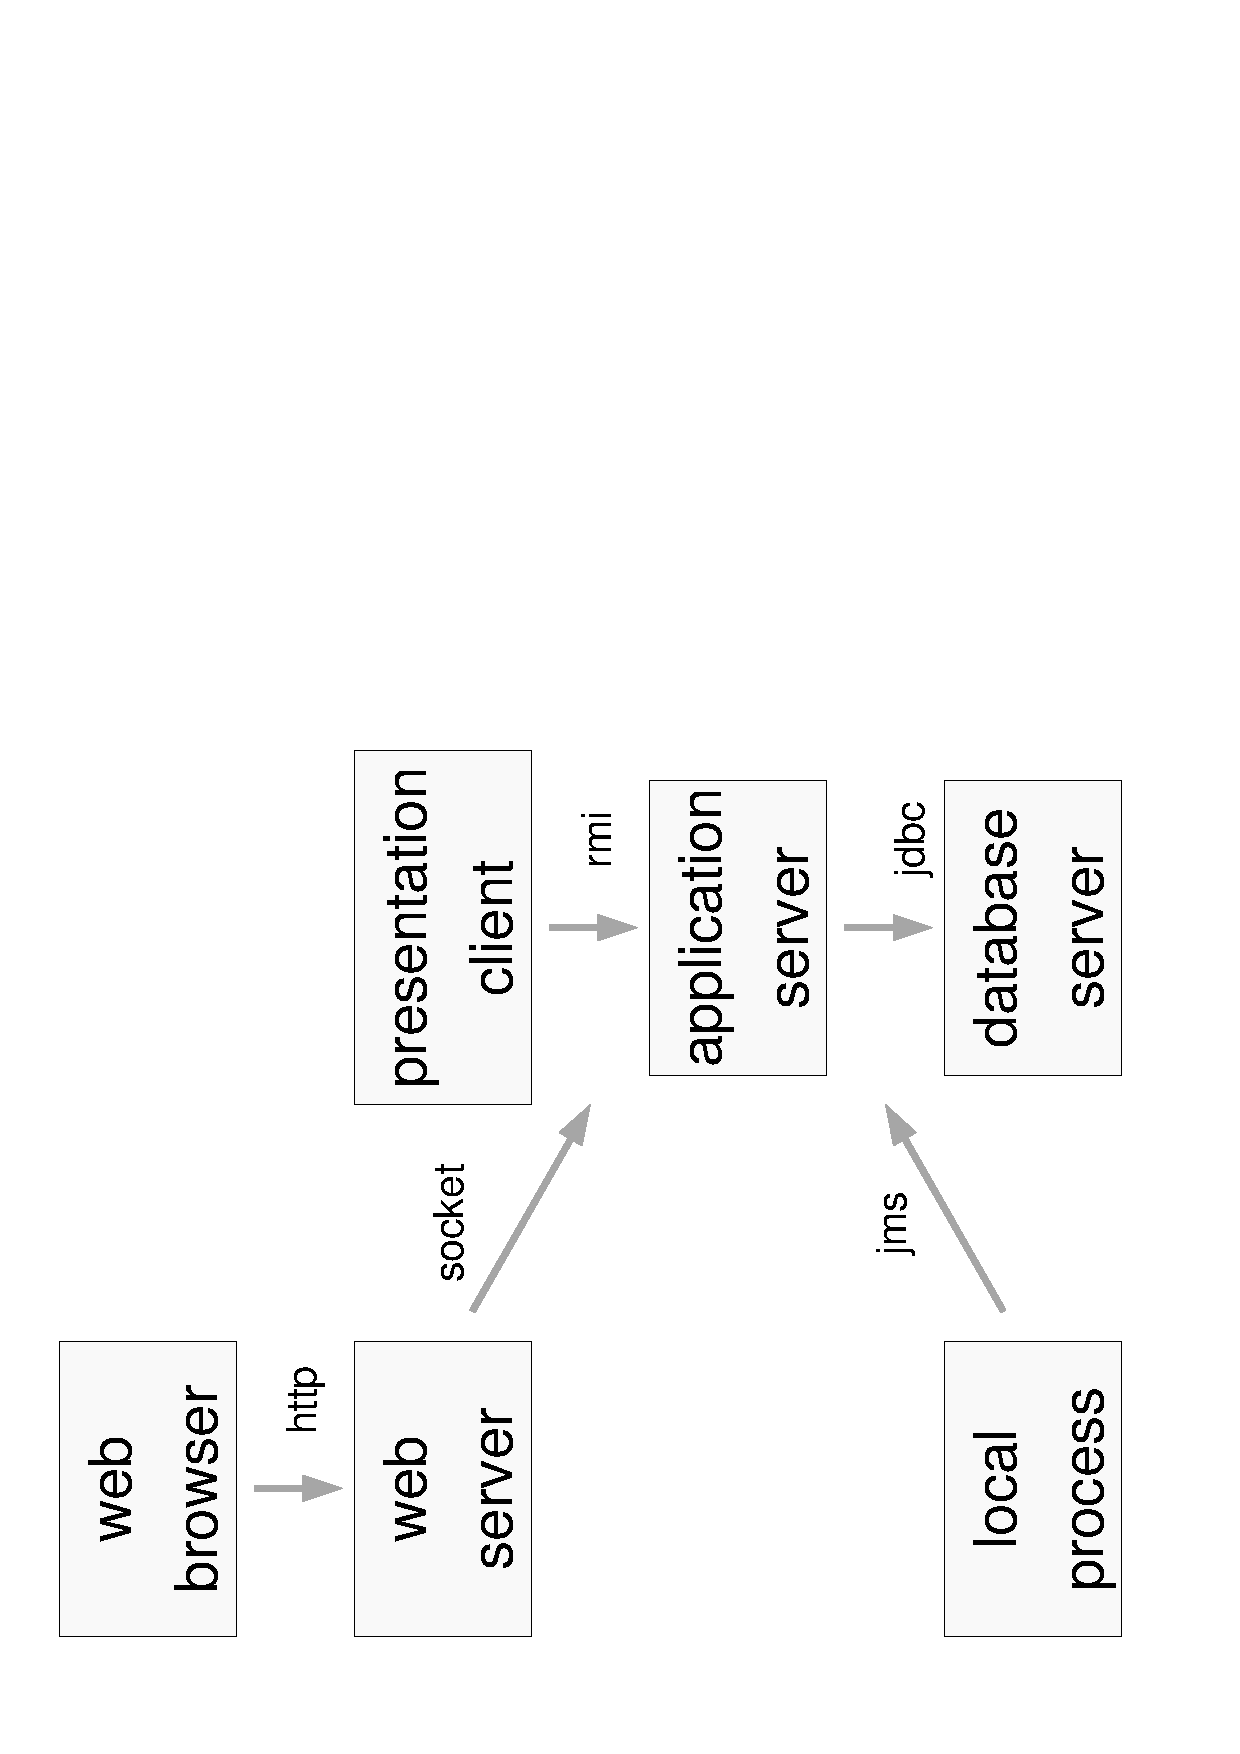
\includegraphics[scale=0.3,angle=-90]{graphic/local.pdf}
        \caption{Local Process}
        \label{local_figure}
    \end{center}
\end{figure}

Sometimes, local processes are needed by the operating system itself. Those are
running in the background then which is why they are often called \emph{Daemon}.
Because they offer special services, daemons are nothing else than small
servers. They fulfil tasks like managing all printing or email delivery of a
system, or similar things \cite[p. 74]{tanenbaum2001}.

Very often, it is useful to let local client applications talk with each other.
One part of a document (for instance a diagram) that was created by help of a
special application may want to get integrated into another document (for instance
a letter) which is edited by another application. A number of mechanisms were
created to solve this \emph{Inter-Process Communication} (IPC) task, for example:

\begin{itemize}
    \item[-] \emph{Dynamic Data Exchange} (DDE) \cite{ddefaq}
    \item[-] \emph{Object Linking and Embedding} (OLE/ OLE2) and \emph{ActiveX},
        both now based on the \emph{Component Object Model} (COM)
        \cite{zimmermann, gruhn}
    \item[-] \emph{Java Message Service} (JMS) \cite{java}
    \item[-] \emph{Desktop Communication Protocol} (DCOP) \cite{kde}
    \item[-] \emph{Bonobo} \cite{gnome}
    \item[-] \emph{Pipes} \cite{johnson, tanenbaum2001}
\end{itemize}

Although usually used for local communication (on the same node), some of these
also function over network. Again, this document will not discuss their inside
functionality. Plenty of books were written about that.
